\documentclass[titlepage]{article}

\usepackage[margin=1in]{geometry}
\usepackage{csquotes}
\usepackage{fancyhdr}
\usepackage{marginnote}
\usepackage{enumitem}
\usepackage{xr}
\usepackage{scrextend}
\usepackage[bottom]{footmisc}
\usepackage[style=chem-acs]{biblatex}
\usepackage{float,subcaption}
\usepackage{graphicx}
\usepackage{tikz}
\usepackage{siunitx}
\usepackage{amsmath,amssymb}
\usepackage{bm}
\usepackage{mhchem,chemfig,chemmacros}
\usepackage[hidelinks]{hyperref}

\MakeOuterQuote{"}

\fancypagestyle{main}{
    \fancyhf{}
    \fancyhead[L]{\leftmark}
    \fancyhead[R]{CHEM 22100}
    \fancyfoot[R]{Labalme\ \thepage}
}
\fancypagestyle{plain}{
    \fancyhead{}
    \renewcommand{\headrulewidth}{0pt}
}

\reversemarginpar

\setitemize[3]{label={\scriptsize$\blacksquare$}}

\deffootnotemark{\textsuperscript{\textup{[}\thefootnotemark\textup{]}}}
\deffootnote[2.1em]{0em}{0em}{\textsuperscript{\thefootnote}}

\DefineBibliographyStrings{english}{bibliography={References}}

\usetikzlibrary{decorations,arrows.meta,bending,calc,decorations.pathreplacing}
\colorlet{rex}{magenta}
\colorlet{gax}{gray!50}
\colorlet{orx}{orange!90!yellow!95!black!90}
\colorlet{blx}{cyan}
\colorlet{grx}{green!60!cyan}

\sisetup{range-phrase=-,range-units=single}
\DeclareSIUnit{\calorie}{cal}
\DeclareSIUnit{\atomicmassunit}{amu}

\setchemfig{atom sep=2em,fixed length=true,bond offset=3pt,cram width=3pt}
\setcharge{extra sep=3pt}
\pgfdeclaredecoration{ddbond}{initial}{
    \state{initial}[width=3.5pt]{
        \pgfpathlineto{\pgfpoint{4pt}{0pt}}
        \pgfpathmoveto{\pgfpoint{0pt}{2pt}}
        \pgfpathlineto{\pgfpoint{1pt}{2pt}}
        \pgfpathmoveto{\pgfpoint{3pt}{2pt}}
        \pgfpathlineto{\pgfpoint{4pt}{2pt}}
        \pgfpathmoveto{\pgfpoint{4pt}{0pt}}
    }
    \state{final}{
        \pgfpathlineto{\pgfpointdecoratedpathlast}
    }
}
\tikzset{
    lddbond/.style={decorate,decoration=ddbond},
    rddbond/.style={decorate,decoration={ddbond,mirror}}
}

\newcommand{\N}{\mathbb{N}}
\newcommand{\e}[1][]{\text{e}^{#1}}

\usepackage{subfiles}

\addbibresource{../../main.bib}

\title{Spectral Analysis of Unknown G}
\author{
    Steven Labalme\\
    \normalsize Lab Section 1A05
}

\begin{document}




\maketitle



\pagestyle{main}
\renewcommand{\leftmark}{Written Assignment 2}
\setitemize{label={--}}
\noindent What is the letter/number of your unknown?
\begin{itemize}
    \item Unknown G.
\end{itemize}



\section*{MS Data}
\begin{enumerate}
    \item What is the molecular weight of the molecular ion (M+), and therefore the molecular weight of your unknown?
    \begin{itemize}
        \item The molecular weight of the molecular ion is $\SI{112}{\atomicmassunit}$.
    \end{itemize}
    \item Does your unknown contain any \ce{Br} atoms? \ce{Cl}? Odd number of \ce{N}? Why or why not?
    \begin{itemize}
        \item It does contain at least one \ce{Cl} atom since there is a peak at $\text{M}+2$ in an approximately $1:3$ ratio with the peak at M.
        \item There is no bromine atom because having a \ce{{}^35Cl} and \ce{{}^79Br} would necessitate an M peak of 114 with $\text{M}+2$ and $\text{M}+4$ peaks due to isotope effects; these latter two are not observed.
        \item There is not an odd number of \ce{N} because the molecular ion peak is at an even value of $m/z$.
    \end{itemize}
    \item Give a molecular formula for your product if it contains no oxygens. Give the molecular formulas if your product contains one or two oxygens (some may not be possible).
    \begin{itemize}
        \item No oxygens: \ce{C6H5Cl}. Minus the chlorine, the molecular weight is 77. This must be \ce{C6H5}, since even a completely unsaturated \ce{C5H11} would only make it to 71.
        \item One oxygen: \ce{C5HClO}. This is highly unlikely though.
        \item Two oxygens: Not possible. We would have to have at most three carbons, and \ce{C3H9O2Cl} is oversaturated.
    \end{itemize}
    \item Calculate the index of hydrogen deficiency, and therefore the number of rings and/or $\pi$-bonds in your unknown for each of the molecular formulas in Question 3. Show your calculations.
    \begin{itemize}
        \item No oxygens:
        \begin{equation*}
            \frac{(2\cdot 6+2)-5\cdot 1-1\cdot 1}{2} = 4
        \end{equation*}
        \item One oxygen:
        \begin{equation*}
            \frac{(2\cdot 5+2)-1\cdot 1-1\cdot 1-0\cdot 1}{2} = 5
        \end{equation*}
    \end{itemize}
\end{enumerate}



\section*{IR Data}
\begin{enumerate}
    \item Is there a carbonyl in your unknown? State how you know. If one is present, state how the frequency narrows down the functional group it is a part of (carboxylic acid, ketone, aldehyde, ester, amide).
    \begin{itemize}
        \item No. There is not a significant peak in the viscinity of \SI{1710}{\per\centi\meter}.
    \end{itemize}
    \item What functional groups are present in your unknown molecule? For each, correlate the functional group with the frequency of the identifying peak.
    \begin{itemize}
        \item An aromatic ring (peaks at \SI{1470}{\per\centi\meter} and \SI{1584}{\per\centi\meter}).
        \item A \ce{C-H} on an $sp^2$-hybridized carbon (peak at \SI{3059}{\per\centi\meter}).
    \end{itemize}
    \item For each of the molecular formulas you listed in Question 3 of the MS Data section, state if these functional groups support or rule out the formula.
    \begin{itemize}
        \item The lack of an alcohol or carbonyl supports the no-oxygen formula and rules out the one-oxygen formula.
    \end{itemize}
    \item List all the IR data from Questions 1 and 2 in ACS journal style. The format is: IR $\nu$max (ATR) \emph{list major peaks here} \si{\per\centi\meter}.
    \begin{itemize}
        \item IR $\nu$max (ATR) \num{1470}, \num{1584}, \num{1710} \si{\per\centi\meter}.
    \end{itemize}
\end{enumerate}



\section*{\ce{{}^13C} NMR Data}
\begin{enumerate}
    \item Identify the solvent peak in the spectrum and list its chemical shift.
    \begin{itemize}
        \item There is a \ce{CDCl3} peak at $\delta$ 77.
    \end{itemize}
    \item Other than the solvent peak, how many signals are present in the \ce{{}^13C} NMR and how does this correlate to the number of chemically distinct carbons?
    \begin{itemize}
        \item There are four other signals present in the \ce{{}^13C} NMR, correlating to four chemically distinct carbons.
    \end{itemize}
    \item Based on the chemical shifts, what functional groups are present in your compound? For each, correlate the functional group with the chemical shift of the identifying peak.
    \begin{itemize}
        \item There is an alkene and/or aryl group in this compound. All four peaks (shifts $\delta$ 126, 128, 129, and 134) support this. It should be noted that it is also technically possible that a nitrile group is present, but this is unlikely since there was no indication of one in the IR spectrum.
    \end{itemize}
    \item For each of the molecular formulas you listed in Question 3 in the MS Data section, state if your \ce{{}^13C} NMR data supports or rules out the formula.
    \begin{itemize}
        \item Since, once again, no oxygen-related peaks are present, the \ce{{}^13C} NMR data supports the no-oxygen formula and rules out the one-oxygen formula.
    \end{itemize}
    \item What molecular formula(s) are supported by both the IR and \ce{{}^13C} NMR data?
    \begin{itemize}
        \item The no-oxygen formula is supported by both IR and \ce{{}^13C} NMR.
    \end{itemize}
    \item List all the \ce{{}^13C} NMR data in ACS journal style. The format is: \ce{{}^13C} NMR (\SI{125}{\mega\hertz}, \ce{CDCl3}): $\delta$ \emph{list chemical shifts here}.
    \begin{itemize}
        \item \ce{{}^13C} NMR (\SI{125}{\mega\hertz}, \ce{CDCl3}): $\delta$ 126, 128, 129, 134.
    \end{itemize}
\end{enumerate}



\section*{\ce{{}^1H} NMR Data}
\begin{enumerate}
    \item List the integration of all peaks as a ratio. For example, 4-hydroxy-4-methyl-2-pentanone would have a ratio of $1:2:3:6$. How does the integration of the peaks correlate to the number of hydrogens present in the molecule?
    \begin{itemize}
        \item $1$. It does not give any information since there is only one peak.
    \end{itemize}
    \item For the molecular formula(s) listed in Question 5 of the \ce{{}^13C} NMR Data section, state if the integration data supports or rules out the formula(s).
    \begin{itemize}
        \item It neither supports nor rules out any of the formulas since it doesn't comment on the total amount of hydrogens present.
    \end{itemize}
    \item Based on the chemical shifts, what functional groups are present in your compound? For each, correlate the functional group with the chemical shift of the identifying peak.
    \begin{itemize}
        \item There are one or more aromatic hydrogens in this compound. The one peak present (shift $\delta$ 7.3) support this. It should be noted that it is also technically possible that a phenolic hydrogen is present, but this is unlikely since there was no indication of an oxygen in the IR or \ce{{}^13C} NMR spectrum.
    \end{itemize}
    \item State how the functional groups identified in the \ce{{}^1H} NMR data correlate with the functional groups identified in the \ce{{}^13C} NMR and IR data. If there are any molecular formula(s) ruled out by this data, state that as well.
    \begin{itemize}
        \item This aromatic hydrogen correlates well with the suggestion of an aromatic group or alkene by the IR and \ce{{}^13C} NMR spectra. Additionally, it gives us our first indication that it is an aromatic group present, not just an alkene, as there are no peaks in the alkene region of the \ce{{}^1H} NMR spectrum.
    \end{itemize}
    \item For each peak in the \ce{{}^1H} NMR spectrum, state the splitting pattern and how many neighboring hydrogens this correlates to. Example: singlet - 0 neighboring hydrogens.
    \begin{itemize}
        \item Multiplet.
    \end{itemize}
    \item For each peak, draw a partial structure that uses all three pieces of information (chemical shift, integration, splitting patterns). Make sure that you highlight the hydrogen atom or atoms that are responsible for the signal. An example of this is \ce{-R-CO-C\textbf{H}2-R} or
    \begin{center}
        \footnotesize
        \chemfig{R-[:30](=[2]O)-[:-30](-[:-70]\textbf{H})(-[:-110]\textbf{H})-[:30]R}
    \end{center}
    \begin{itemize}
        \item There exists a monosubstituted aromatic ring:
        \begin{center}
            \chemfig{*6(-=-=(-Y)-=)}
        \end{center}
    \end{itemize}
    \item List all the \ce{{}^1H} NMR data in ACS journal style. The format is: \ce{{}^1H} NMR (\SI{500}{\mega\hertz}, \ce{CDCl3}): $\delta$ \emph{chemical shift} (\emph{splitting}, \emph{integration}). As an example, the following peak would be reported as: \ce{{}^1H} NMR (\SI{80}{\mega\hertz}, \ce{CDCl3}): $\delta$ 1.75 (sextet, 2H)
    \begin{center}
        \begin{tikzpicture}
            \draw [ultra thick] (0,0) -- (3,0);
            \draw [gray]
                (0.5,0) node[below,black]{\LARGE 2} -- ++(0,4.5)
                (0,4) -- ++(3,0)
                (0,3) -- ++(3,0)
                (0,2) -- ++(3,0)
                (0,1) -- ++(3,0)
            ;
    
            \draw [thick] (0,0.2)
                -- (1.30,0.20)
                -- (1.35,0.60)
                -- (1.40,0.25)
                -- (1.45,2.15)
                -- (1.50,0.35)
                -- (1.55,3.90)
                -- (1.60,0.40)
                -- (1.65,3.80)
                -- (1.70,0.35)
                -- (1.75,2.20)
                -- (1.80,0.25)
                -- (1.85,0.65)
                -- (1.90,0.20)
                -- (3.00,0.20)
            ;
        \end{tikzpicture}
    \end{center}
    \begin{itemize}
        \item \ce{{}^1H} NMR (\SI{500}{\mega\hertz}, \ce{CDCl3}): $\delta$ 7.3 (multiplet, 5H).
    \end{itemize}
\end{enumerate}



\section*{Final Structure}
\begin{enumerate}
    \item Piece together a complete structure of your unknown using everything that you have listed so far into a drawing using chemical drawing software.
    \begin{center}
        \chemfig{*6(-=-=(-Cl)-=)}
    \end{center}
    \item Locate published IR and \ce{{}^1H} NMR spectra for your proposed structure and compare them to the spectra you received. Discuss why these published spectra prove the identity of your unknown or disprove your proposed structure. Be sure to correlate all data referenced in the IR and \ce{{}^1H} NMR sections. Include the spectra and citations in your report.
    \begin{figure}[h!]
        \centering
        \begin{subfigure}[b]{0.8\linewidth}
            \centering
            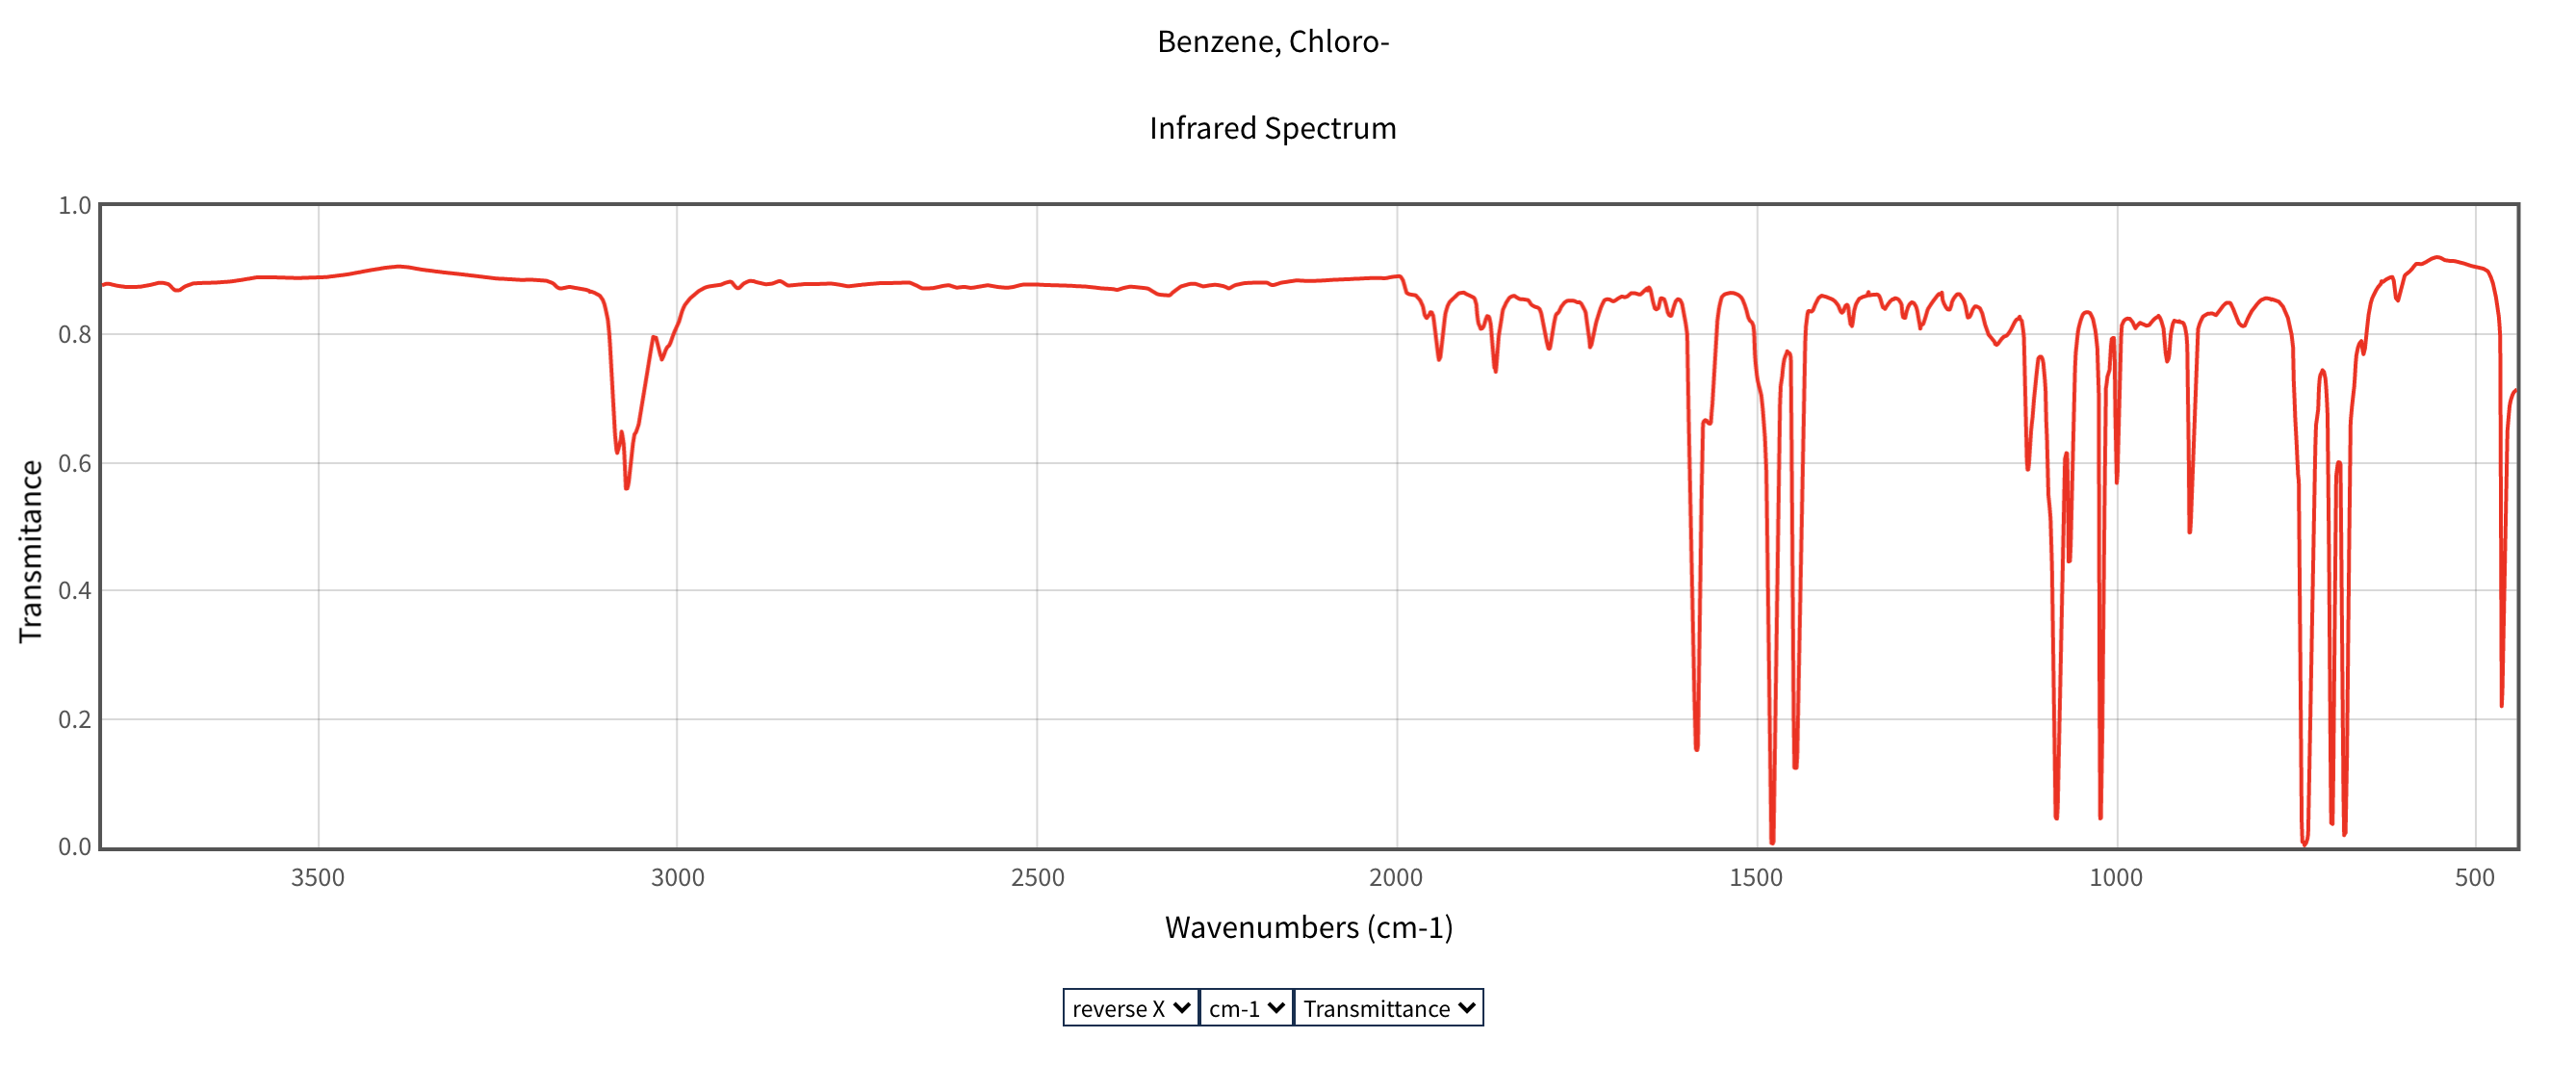
\includegraphics[width=0.9\textwidth]{../../ExtFiles/Chlorobenzene-IR.png}
            \caption{IR spectrum.}
            \label{fig:spectraa}
        \end{subfigure}\\[1em]
        \begin{subfigure}[b]{0.4\linewidth}
            \centering
            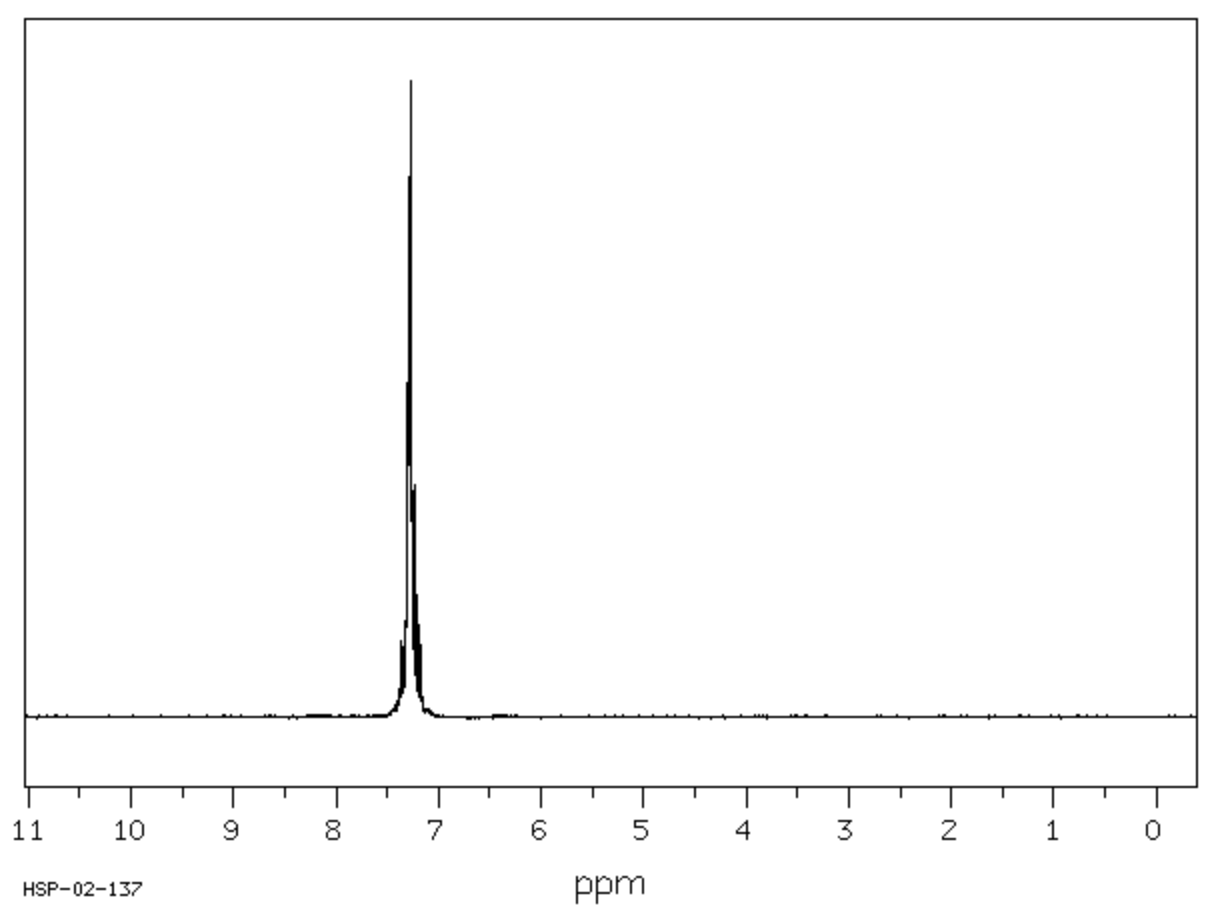
\includegraphics[width=0.9\textwidth]{../../ExtFiles/Chlorobenzene-1HNMR.png}
            \caption{\ce{{}^1H} NMR spectrum.}
            \label{fig:spectrab}
        \end{subfigure}
        \caption{Spectra of the proposed compound.}
        \label{fig:spectra}
    \end{figure}
    \begin{itemize}
        \item Both the IR spectrum\supercite{bib:Chlorobenzene-IR} and the \ce{{}^1H} NMR spectrum\supercite{bib:Chlorobenzene-1HNMR} I found exactly match the peaks I noted earlier (and, in the case of the IR spectrum, the fingerprint region). In particular, IR peaks at 1470, 1584, and \SI{1710}{\per\centi\meter} and a single \ce{{}^1H} NMR signal at $\delta$ 7.3 predominate in both respective spectra.
    \end{itemize}
\end{enumerate}
\newpage



\printbibliography




\end{document}